\documentclass{article}
\usepackage[utf8]{inputenc}

\usepackage{listings}
\usepackage{color}
\usepackage{graphicx}

\definecolor{dkgreen}{rgb}{0,0.6,0}
\definecolor{gray}{rgb}{0.5,0.5,0.5}
\definecolor{mauve}{rgb}{0.58,0,0.82}

\lstset{frame=tb,
  language=Java,
  aboveskip=3mm,
  belowskip=3mm,
  showstringspaces=false,
  columns=flexible,
  basicstyle={\small\ttfamily},
  numbers=none,
  numberstyle=\tiny\color{gray},
  keywordstyle=\color{blue},
  commentstyle=\color{dkgreen},
  stringstyle=\color{mauve},
  breaklines=true,
  breakatwhitespace=true
  tabsize=3
}


\title{Reversi Online Design Documentation}
\author{Patrick Rock}
\date{October 2013}

\begin{document}

\maketitle

\section{Introduction}
Reversi is an old strategy game played on an 8x8 board. We will be implementing
an online version of the game in Java. Our implementation will feature a GUI and a simple
min-max AI. The project will be done in three major releases: server, AI, and GUI.
We will be using Github and Pivotal Tracker to manage the project. Pivotal Tracker
is an online tool that helps manage SCRUM Backlogs.

\section{Game Rules}
Developing a game requires a strong understanding of the rules. These rules will
be implemented by a class, the Game Engine.
Two players compete to have the most pieces on the board. 
The game ends when neither player can move.
The players take turns unless one player can't make a valid move. 
The dark player moves first.
Dark must play on a square with a straight occupied line to another dark piece. There 
must be at least one white piece in between them. Dark captures the white pieces
on the line.

\section{High Level Design}
The following are classes in our application:
\begin{itemize}
\item Game State   - Represents a valid configuration of the Reversi board
\item Location     - Represents a coordinate on the game board
\item Game Engine  - Handles game flow, changing game state, and AI
\item Parser       - Reads commands in the network protocol 
\item GUI          - Renders interface, will have many subclasses for board, menu, etc...
\item Server       - Controller class
\item Client       - Connects to Server over telnet
\item 
\end{itemize}

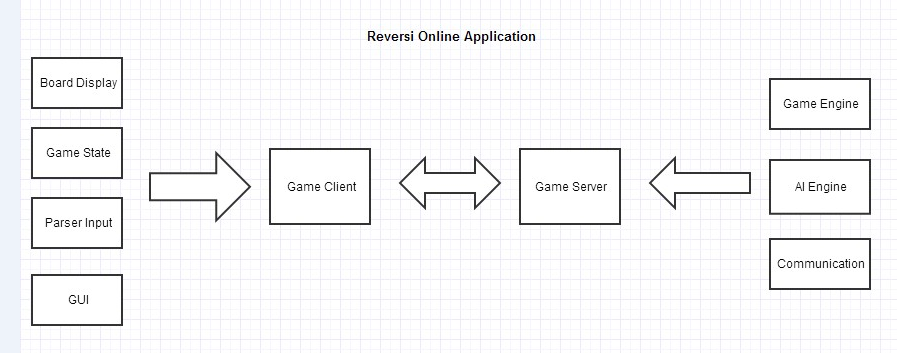
\includegraphics[scale=0.4]{HighLvlDesign.png}

\section{Low Level Design}

\subsection{Game State}
The reversi board is an 8x8 grid. We will represent the board with an 8x8 matrix, each position
in the matrix will contain a piece object. A piece object is white or black.
The Game State is a simple wrapper for a matrix.
The AI must also build a tree where each node represents a state of the game. Having an explicit
state class will simplify the min max process.    

\subsection{Game Engine}
The purpose of the game engine is to handle the high level flow of the game. The engine
can control human vs human, and human vs AI games. It has public methods move() and aiMove().
The engine should have private methods, isValid(state) to check for valid game states, and isOver(state)
to check for end game states. The AI component will have a heuristic function which evaluates a given game
state. This is used to weight the min max tree. The Engine exposes the interface:
\begin{itemize}
\item int move(loc1, loc2) 
\item int aiMove()
\end{itemize}

\subsection{Parser}
The parser reads text conforming to the network protocol and traslates into Game Engine actions.
The parser will use recursive descent and a token of lookahead. The parser is an abstract class,
the subclasses ServerParser and Client Parser will each implement a different grammar. A parser
object simply calls parse(string) on a command.
The grammar of the ServerParser is:
\begin{verbatim}
expr     ::= command | move | comment
command 
  
 	 ::= EXIT | DISPLAY 
| difficulty 
| UNDO 
| HUMAN-AI|AI-AI <server> <port> difficulty difficulty
difficulty	 ::= EASY|MEDIUM|HARD
move	 ::= column row
comment	 ::= ; *
column	 ::= a | b | c | d | e | f | g | h
row	 ::= 1 | 2 | 3 | 4 | 5 | 6 | 7 | 8
digit	 ::= 0 | 1 | 2 | 3 | 4 | 5 | 6 | 7 | 8 | 9
server	 ::= IP address or hostname
port	 ::= digit { digit }
\end{verbatim}

\vspace{10 mm}
The grammar of the ClientParser is:
\begin{verbatim}
ack	 ::= WELCOME | OK | move | ILLEGAL | comment
move	 ::= column row
column	 ::= a | b | c | d | e | f | g | h
row	 ::= 1 | 2 | 3 | 4 | 5 | 6 | 7 | 8
comment	 ::= ; *
\end{verbatim}

Each parser should built in two phases. First recognize the grammar correctly, then 
tie the production rules to actions in the Game Engine.


\subsection{GUI}
Since we are building our application in Java, we will use Swing to build 
our GUI. We may take advantage of swing concurrency depending on how 
smoothly the project goes. 

\subsection{Server}
The server must parse incomming data from the client and respond.
Before the GUI is implemented the Server shold display a plaintext representation 
of the gameboard. This functionality could be offloaded into the Game Board object.
The Game Engine will run inside the Server. The server will also contain the networking
socket code. The server's main loop depends on what sort of game is being played. There 
will be a server function for each game type which enters the main loop.

\subsection{Client}
The client must parse data from the server and respond. The client will also
implement the GUI. Java Swing uses the idea of a containment hierarchy. The application
contains drawable entities, which themselves may contain drawables. Our application will contain
a menu cass and a board class. The menu class will bee an instance of JMenu.

\section{Conclusion} % benefits, assumptions, risks/issues
The benefits of this project : 
\begin{itemize}
\item this Reversi Online game has several modes to play: Human vs Human; Human vs AI; AI vs AI. 
\item This game has GUI which is easy to play
\item Different AI settings allow user to vary the difficulty
\end{itemize}
Assuptions:
\begin{itemize}
\item Assumes the network is working 
\item Assumes the server runs in Unix environment and client runs in a graphical environment
\item Assumes the Java Swing is the right choice for building out GUI
\end{itemize}
Risks: Java GUI has to run in the  graphical environment, otherwise, user can’t play this game
\end{document}

